\section{Packet Routing with In-network Processing}
\label{sec:routing}
%%%%%%%%%%%%%%%%%%%
%%%%%%%%%%%
%Basic problem
%%%%%%%%%%%
%%%%%%%%%%%%%%%%%%
\subsection{The basic problem}
\label{subsec:basicproblem}
We begin by introducing the routing problem in the presence of processing demands. In this problem, we are given a directed graph $G = (V,E)$ along with edge capacities $B : E \rightarrow \positivereal$, vertex capacities $C : V \rightarrow \nonnegativereal$, and a collection of demanded integer flows $D = \{(s_1, t_1, k_1), (s_2, t_2, k_2), \cdots\} \subseteq V \times V \times \positivereal$. While the edge capacities are used in a manner entirely analogous to its uses in standard multicommodity flow problems, we also require that each unit of flow undergo one unit of processing at an intermediate vertex. In particular, while edge capacities limit the \textit{total} amount of flow that may pass through an edge, vertex capacities only bottleneck the amount of processing that may be done at a given vertex, regardless of the total amount of flow that uses the vertex as an intermediate node. The goal is then either to route as much flow as possible, or to satisfy all flow demand subject to appropriate congestion-minimization objective function. Though ignoring vertex capacity constraints reduces our class of problems to those of the standard Multicommodity Flow variety, the introduction of these constraints forms a new class of problems that (to our knowledge) has not yet been studied in the literature.

\begin{figure}
\centering
  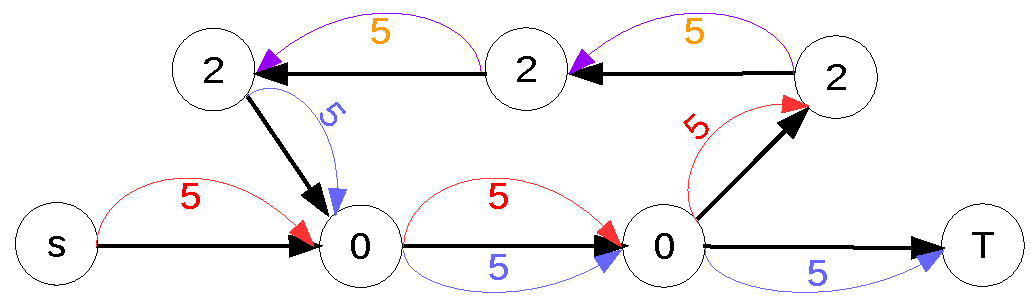
\includegraphics[width=0.7\linewidth]{images/demo2.pdf}
 \caption{The edge capacity is 10 for all edges and the node capacities are denoted in each node. Here, we can send maximum flow size 5, by routing it along the red arcs, have it processed at the nodes at the top, and then sent to $T$ along the blue arcs. The capacity of the bottom middle edge forms the bottleneck here, as all flow must pass through it twice before reaching $T$.}
\end{figure}

\subsubsection{Flow Maximization}
\label{sec:flowmax}
We begin by showing how to express the maximization version of the problem both as an \textit{edge-based} and as a \textit{walk-based} linear program. While neither of these constructions is particularly difficult, it is not obvious that either is enough to solve the flow problem in polynomial time. In particular, while the walk-based LP requires exponential size, the polynomial-sized edge-based LP may a-priori not correspond to valid routing pattern at all. In \autoref{subsec:lppaths}, we resolve this problem by showing that the two linear programs are equivalent, and so the edge-based LP inherits the correctness of the walk-based program, ensuring that we can indeed find a valid solution in polynomial time. We summarize this result in the following theorem.

\begin{theorem}
\label{thm:flowmax}
There exists a polynomial-sized linear program solving the Maximum Processed Flow problem. Further, the full routing pattern can be extracted from the LP solution by decomposing it into its composing $s_i, t_i$ walks in $O(|V| \cdot |E| \cdot |D|)$ time.
\end{theorem}

To express the walk-based linear program, we require one variable $p_{i,\pi}^v$ for each walk-vertex-demand triplet, representing the total amount of flow from $s_i,t_i$ exactly utilizing walk $\pi$ and processed at $v$. The aggregate $(s_i,t_i)$ flow sent along a given walk $\pi$ is then simply denoted by $p_{i,\pi}$, and the set of all walks is given by $P$. The linear program is then the standard multicommodity-flow LP augmented with the new processing capacity constraints.

The edge-based formulation can be thought of as sending two flows for each $D_i$: $f_i$ represents the packets being sent from $s_i$ to $t_i$ and $w_i$ is the processing demand of these packets. While $f_i$ is absorbed (non-conserved) only at the terminals, $w_i$ is absorbed only at the processing vertices. The variables $f_i(e)$ and $w_i(e)$ measure how much of $f_i$ and $w_i$ passes through edge $e$. We use the notation $\delta^+(v)$ and $\delta^-(v)$ to denote the edges leaving and entering vertex $v$, respectively. The two linear programs are given below:
\newline
\begin{minipage}[t]{0.45\textwidth}
\textit{Walk-based formulation:}
\small
  \begin{subequations}
\begin{align*}
&\textsc{maximize }& \sum_{i=1}^{|D|}\sum_{\pi \in P}p_{i,\pi}
\\  
&\textsc{subject to} \\
& p_{i,\pi} = \sum \limits_{v\in \pi} p_{i,\pi}^v& \forall i \in [|D|], \forall \pi \in P \\
& \sum\limits_{i=1}^{|D|}\sum \limits_{\stackrel{\pi\in P}{\pi \ni e}} p_{i,\pi} \leq B(e) & \forall e \in E\\
&\sum\limits_{i=1}^{|D|} \sum \limits_{\pi\in P} p_{i, \pi}^v \leq C(v) &\forall v \in V \\
&p_{i,\pi}^v \geq 0 \hspace{-.5in} &\forall i\in[|D|],\forall \pi\in P,\forall v \in V
\end{align*}
\end{subequations}
\normalsize
 \end{minipage}
 \hfill
 \hspace{.2in}
  \begin{minipage}[t]{0.45\textwidth}
\textit{Edge-based formulation:}
\small
  \begin{subequations}
\begin{align*}
&\textsc{maximize }&\sum\limits_{i=1}^{|D|}\sum \limits_{e\in \delta^+(s_i)} f_i(e)  \\ 
&\textsc{Subject to}\\%\hspace{-.19in}
&\sum\limits_{e \in \delta^-(v)}  f_i(e)=  \sum\limits_{e \in \delta^+(v)} f_i(e)& \forall i \in [|D|], \forall v \in V \setminus \{s_i,t_i\}\\
&p_i(v) = \sum\limits_{e \in \delta^-(v)} w_i(e) - \sum\limits_{e \in \delta^+(v)} w_i(e)  \hspace{-.3in}&\forall i \in [|D|],\forall v \in V\\
&\sum\limits_{i=1}^{[D]} f_i(e)\leq B(e)&\forall e \in E\\
&\sum\limits_{i=1}^{|D|} p_i(v) \leq C(v)&\forall v \in V\\
&w_i(e) \leq f_i(e)  &\forall i \in [D], \forall e \in E \\
&w_i (e)= f_i (e)&\forall i \in [D],\forall e \in \delta^+(s_i) \\
&w_i (e)= 0&\forall i \in [D], \forall e \in \delta^-(t_i) \\
&w_i (e), p_i (v) \geq 0&\forall i \in [D],\forall e \in E 
\end{align*}
\end{subequations}
\normalsize
\end{minipage}
%\ \\

\paragraph{Flow Maximization with Size Changes}
In some cases, middlebox processing might significantly alter the volume of data in a given connection. For example, encrypting middleboxes might increase the size of the flow, while compression and transcoding may substantially decrease it \cite{CDL99}. If processing scales the size of the data of flow $i$ by a constant multiplicative factor $r_i \in \positivereal$, such effects can be captured by linear programs. To do so, we need to separate the flow into two types, preprocessed and postprocessed, which can be represented as $w$ and $f-w$. The increase of postprocessed flow equals the decrease of preprocessed flow. So the flow conservation constraint of the original edge-based LP should be replaced by $ p_i(v) \cdot r_i = \sum_{e \in \delta^+(v)} (f_i(e) - w_i(e)) - \sum_{e \in \delta^-(v)} (f_i(e) - w_i(e))$. 

%If for flow $i$ there is a size change factor $r_i\in \nonnegativereal$, at each vertex, we have $\sum\limits_{in} w_i(e) - \sum\limits_{out}  w_i(e) = p_i(v)$ and $\sum\limits_{out} (f_i(e) - w_i(e))-\sum\limits_{in}  (f_i(e) - w_i(e))= p_i(v)*r_i$, . If $r_i=1$, we have exactly the flow conservation $\sum\limits_{out} f_i(e) -\sum\limits_{in}  f_i(e)= 0$. 

\subsubsection{Cost Minimization}
The minimization version of our problem, however, allows for nonlinear (and, in principle, non-convex) objective functions. In this paper, we deal with the \textit{minimum congestion} model, parameterized by two monotone, convex congestion measures $c_v : \nonnegativereal \rightarrow \nonnegativereal$ and $c_e : \nonnegativereal \rightarrow \nonnegativereal$. In this model, a vertex $v$ with processing capacity $C(v)$ is assigned a congestion $c_v = c_v(\frac{\sum_{f \in F} f_v}{C(v)})$ and each edge is assigned congestion $c_e  = c_e(\frac{\sum_{f \in F} f_e}{B(e)})$, where $f_v$ and $f_e$ are the amount of processing and amount of flow that flow path $f$ assigns to vertices $v$ and $e$, respectively. Each \textit{{flow}}, in turn, is penalized according to the total amount of congestion it encounters among the edges it takes as well as its processing vertex. The goal is to feasibly route all requested units of flow while minimizing the sum of the penalties the various {flow} encounter, or, equivalently, to minimize $\sum_{e \in E} c_e f_e + \sum_{v \in V} c_v f_v$. 

%Since we can turn this problem into a maximization problem with linear objectives with only an $\epsilon$ loss in approximation, shouldn't just about any convex combination of penalties in the objective function be solvable using convex optimization techniques? This captures the minmax problem too, I think... -YN}\comment{Min max is captured by LP already, so yeah this should capture it -KZ}

As a warmup, let's first consider the special case of constant $c_v(\cdot)$ and $c_e(\cdot)$. With these simple functions in place, we can write our objective function as {\sc Minimize} $\sum_v{c_v(\frac{\sum_{f \in F} f_v}{C(v)}) \sum_{f \in F} f_v} + \sum_e{c_e(\frac{\sum_{f \in F} f_e}{B(e)}) \sum_{f \in F} f_e} = \sum_v{\hat{c}_v\sum_{f \in F} f_v} + \sum_e{\hat{c}_e\sum_{f \in F} f_e}$ for some constants $\hat{c}_e$ and $\hat{c}_v$. Adding in the equality $\sum_{e \in \delta^+(S_i)} f_e = D_i$ for each $S_i$ and copying the rest of the edge-based linear program from \Cref{sec:flowmax} completes the linear program. 


% The more interesting case of monotone convex functions with bounded Lipschitz constant $K$ can be handled by adding in a few constraints. Consider an arbitrary edge $e = (u,v)$ with monotone, convex cost function $c_e(\sum_{f \in F} f_e)$. Let $q$ be some positive integer, $G_e(x) = \int_0^x f(e)$, and let $g_e(i) = G_e^{-1}(\tfrac{i}{qG_{e}(B(e)})$ (that is, $g_e(i)$ finds the amount of flow necessary at $e$ for $c_e$ to equal exactly $(i/q)G_e(B(e))$. Subdividing $e$ into $q$ edges $e_1, e_2, \cdots, e_q$ from $u$ to $v$ with capacities $C(e_i) = g_e(i) - g_e(i-1)$

The more interesting case is monotone convex functions with bounded second derivative. Consider an arbitrary edge $e = (u,v)$ with monotone, convex cost function $c_e(\cdot)$ whose second derivative is bounded by some $K$. Dividing $e$ into $q$ edges $e_1, e_2, \cdots, e_q$ from $u$ to $v$ with capacity $B(e)/q$ and constant cost functions $c_{e_i}(\cdot) = c_e\left(\tfrac{i-.5}{q B(e)}\right)$, we get an edge set which would collectively lower bound the cost incurred by the congestion at $e$. Standard bounds on the errors of Riemman sums show that this error is bounded by $O\left(\tfrac{K}{q^2}\right)$. Thus, selecting $q = \tfrac{\sqrt{K}}{|E|\epsilon}$, the sum of all error terms is bounded by $O(\epsilon)$, giving an additive $O(\epsilon)$ approximation. Thus, complicated functions can be simulated by a collection of constant-congestion edges. A similar technique involving replacing vertices with independent sets lets us replace their cost functions with a collection of constant functions. Thus, if the maximum second derivative $\hat{K}$ over all $c_e$ and $c_v$ is $O(\poly(n))$, this technique gives an additive FPTAS for computing the minimum-cost routing solution.

%%%%%%%%%%%%%%%%%%%
%%%%%%%%%%%
%Mutiple tasks as a DAG
%%%%%%%%%%%
%%%%%%%%%%%%%%%%%%
\begin{figure}
	\centering
 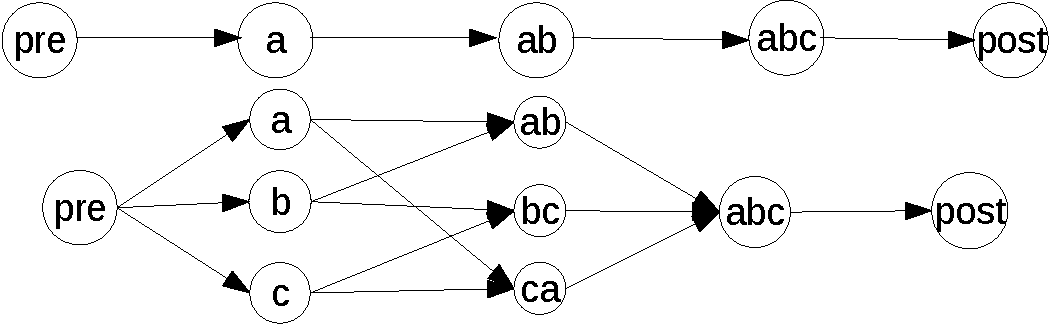
\includegraphics[width=.8\linewidth]{images/task.pdf}
 \caption{Up: Tasks may have strong dependencies and require sequential processing. Down: Tasks may be processible in any order.}
\end{figure}

\subsection{Multiple Types of in-Network Processing as a DAG}
\label{sec:dagrouting}
Sometimes packets need to be processed in multiple, distinct stages. For example, onion routing requires the data to visit a number of intermediaries, each with its own decryption key, before reaching its ultimate destination. Further, it might be the case that certain nodes are fit for only certain types of computations, some of which may contain interdependencies, such as decrypting of files after they pass through a firewall, or encypting a file after it's compressed. Thus, it is natural to attempt to generalize the above formulation into one that can handle multiple processing nodes.

One way to model this type of problem is via DAGs. For each $s_i,t_i$ pair, we require a DAG $G_i$ on vertices $T \subseteq V$. We then require the $s_i, t_i$ flow visit and be processed by nodes in $G_i$ such that processing of $f_i$ at a vertex $v$ succeeding $u$ in $G_i$ is only done after $u$ completed its processing of $f_i$. While in the dependency routing version of the problem we require \textit{all} vertices in the DAG eventually process $f_i$, the {indifference routing} version simply requires $f_i$ to fully traverse and receive processing at each of the vertices on one maximal path in $G_i$. Note that {indifference routing} fully captures the original routing problem from \Cref{subsec:basicproblem} when all intermediary nodes of the DAG form an antichain. 

Interestingly, we can encode both {indifference routing} and {dependency routing} into the above edge-based linear program, though the latter may require an exponential number of new constraints. To do so, each vertex $v$ needs to be given $T$ different processing capacities $C_1(v) \cdots C_{T}(v)$, one for each task. {Indifference routing} can then be implemented by replacing each $w_i(e)$ with a collection of $w_i^t(e)$ measuring how much processing of task $t$ the $(s_i, t_i)$ flow along $e$ yet demands and adding in simple inequalities ensuring that the flow processed by $v$ is no more than the sum of all flows processed on $v$'s immediate predecessors in $G_i$. The straightforward approach to ensuring feasibility in the {dependency routing} case, however, requires flows to fully identify their processing history to ensure that multiple fractionally-processed flows don't get merged and counted as a fully processed flow by the LP. We then ensure that any processing done by vertex $u$ only be done on flow that identifies itself as having been processed at each of $u$'s immediate predecessors. Although the naive encoding requires up to $2^T$ new flows be created for each $(s_i, t_i)$ pair, it is sufficient to decompose $T$ into a chains and store the progress of the processing along each chain using at most $\log T$ bits per chain. A simple application of Dilworth's Theorem\cite{Dilworth} allows us to bound the size of this encoding by $2^{A(G_i)} \log |T| = |T| 2^{A(G_i)}$, where $A(G_i)$ is the size of the largest antichain in $G_i$. This gives a significant advantage when the interdependency poset is close to a chain. %It can be shown by Dillworth's theorem%In optimization formulation above $f$ and $w$ can be interpreted as two different flow states, pre-processed with volume $w$ and post-processed $f-w$.  In \emph{serial model} we have $N+1$ flow states: pre-$n$-post-$(n-1)$ processed where $ n\in\{1\dots N+1\}$. We can extend formulation by adding $N-1$ process demands, in particular for $p_i$ we extend to N different types of processing, $p_i^n= \sum\limits_{in} w_i^n(e) - \sum\limits_{out} w_i^n(e)$. Besides the same capacity and flow relation constraints, we also need $w_i^n(e) \geq w_i^{n-1}(e)$ where it reflects the order. The complexity of this formulation increases in a linear relation to the number of tasks $N$. 

%In the above formulation we assume either there is only one task, or each vertex can run all types of flow processing tasks where we can treat tasks as a single task and simply process them together. Nevertheless if we have specialized hardware for different types of tasks or two types of tasks are preferred at different vertices,  we need to revisit our formulation. 
%We consider two common types of task relationships: \checkthis{ ordered and unordered?}. Ordered tasks must be handled in a certain order while unordered tasks can happen in any order. A set of tasks may require a policy of a mixture of ordered and unordered, e.g., a flow requires three different types of processing a, b and c, and a is before b and c while b and c can happen in either order. 

%We can extract any arbitrary task topology as a partial ordered set (poset). We show two simplest cases where all N tasks are ordered or unordered, then we generalize the solution to any arbitrary order via chain-antichain sets. Example see figure 2.


%For $N$ tasks, we have $C^n(v); n\in\{1\dots N\}$ for $N$ different processing capacities. In optimization formulation above $f$ and $w$ can be interpreted as two different flow states, pre-processed with volume $w$ and post-processed $f-w$.  In \emph{ordered model} we have $N+1$ flow states: pre-$n$-post-$(n-1)$ processed where $ n\in\{1\dots N+1\}$. We can extend formulation by adding $N-1$ process demands, in particular for $p_i$ we extend to N different types of processing, $p_i^n= \sum\limits_{in} w_i^n(e) - \sum\limits_{out} w_i^n(e)$. Besides the same capacity and flow relation constraints, we also need $w_i^n(e) \geq w_i^{n-1}(e)$ where it reflects the order. The complexity of this formulation increases in a linear relation to the number of tasks $N$. 
%In \emph{unordered model} we have $2^N$ processing states and $O(2^N)$ numbers of inequalities for transitioning flow states such as from preprocessed states for cerain tasks to postprocessed states; and $O(N)$ number of inequalities for the vertex capacity.
%In general; for a topology with a maximum number of A antichains and L is the maximum length of a chain, then we need maximum $A \lg L$ bits to presents the states, so we have $2^{A \lg L} = L*2^A$ number of states, in other words, the upper bound of the number of flow states is exponential to the width of the poset, and linear to the height of poset.

%We can satisfy the new requirement by modifying the optimization formulation. We consider two corner cases where there are N serial or N parallel tasks, and then we extend this to a general case where N tasks have a DAG relation. 

%For $N$ serial tasks, we have $C^n(v); n\in\{1\dots N\}$ for $N$ different processing capacities. In optimization formulation 2.2, we can think of two different types of flows, pre-processed and post-processed, and in this model we have $N+1$ types of flows: pre-$n$-post-$(n-1)$ processed where $ n\in\{1\dots N\}$ and  fully processed flows. We can extend formulation 2.2 by adding $N-1$ process demands, in particular for 2.2c we extend to N different types of processing, $p_i^n= \sum\limits_{in} w_i^n(e) - \sum\limits_{out} w_i^n(e)$. Besides the same capacity and flow relation constraints, we also need $w_i^n(e) \geq w_i^{n-1}(e)$ where it reflects the sequence. The complexity of this formulation increases in a linear relation to the number of tasks $N$.


%For $N$ parallel tasks, again we have $C^n(v); n\in\{1\dots N\}$ for $N$ different processing capacities. Unlike serial relation, the number of types of flow grows exponentially, at most there can be $2^N$ types of flows. We have $O(2^N)$ inequalities represents the dependencies and $O(N)$ inequalities represents processing capacity relations.
% Surprisingly the complexity of the formulation also increases in a linear relation to the number of tasks N if we utilize the independence between tasks. The constraints are almost the same as above serial case except for that there is no sequential constraint like $w_i^n(e) \geq w_i^{n-1}(e)$. This optimization problem is similar to solve $N$ separate optimization problems and the $N$ problems are linked by the routing choice $f_i$ and the objective function. We argue that the optimization solution also provides with enough information for routing and processing decision; we can process the flow in the following manner: each flow has $N$ tags which indicates whether the part of the flow $n\in\{1\dots N\}$ is processed, and since the order can be arbitrary for $N$ processings, for each type of processing, it only needs to check its corresponding tag and make decisions independently. 

%To generalize, if there are tasks with a DAG relation where each directed link $(p,q)$ represents a dependency of $q$ to $p$, there is an inequality relation $w_i^q(e) \geq w_i^p(e)$ for each link $(p,q)$. For any k parallel tasks, we need to build $O(2^k)$ branches and establish the relation using the method above.   